\documentclass[12pt, titlepage]{article}

\usepackage{fullpage}
\usepackage[round]{natbib}
\usepackage{multirow}
\usepackage{booktabs}
\usepackage{tabularx}
\usepackage{graphicx}
\usepackage{float}
\usepackage{hyperref}
\hypersetup{
    colorlinks,
    citecolor=blue,
    filecolor=black,
    linkcolor=red,
    urlcolor=blue
}

%% Comments

\usepackage{color}

\newif\ifcomments\commentstrue %displays comments
%\newif\ifcomments\commentsfalse %so that comments do not display

\ifcomments
\newcommand{\authornote}[3]{\textcolor{#1}{[#3 ---#2]}}
\newcommand{\todo}[1]{\textcolor{red}{[TODO: #1]}}
\else
\newcommand{\authornote}[3]{}
\newcommand{\todo}[1]{}
\fi

\newcommand{\wss}[1]{\authornote{blue}{SS}{#1}} 
\newcommand{\plt}[1]{\authornote{magenta}{TPLT}{#1}} %For explanation of the template
\newcommand{\an}[1]{\authornote{cyan}{Author}{#1}}

%% Common Parts

\newcommand{\progname}{SFWRENG 4G06} % PUT YOUR PROGRAM NAME HERE
\newcommand{\authname}{Team 9, dice\_devs
\\ John Popovici
\\ Nigel Moses
\\ Naishan Guo
\\ Hemraj Bhatt
\\ Isaac Giles} % AUTHOR NAMES                  

\usepackage{hyperref}
    \hypersetup{colorlinks=true, linkcolor=blue, citecolor=blue, filecolor=blue,
                urlcolor=blue, unicode=false}
    \urlstyle{same}
                                


\newcounter{acnum}
\newcommand{\actheacnum}{AC\theacnum}
\newcommand{\acref}[1]{AC\ref{#1}}

\newcounter{ucnum}
\newcommand{\uctheucnum}{UC\theucnum}
\newcommand{\uref}[1]{UC\ref{#1}}

\newcounter{mnum}
\newcommand{\mthemnum}{M\themnum}
\newcommand{\mref}[1]{M\ref{#1}}

\begin{document}

\title{Module Guide for \\\progname: \\Dice Duels: Duel of the Eights} 
\author{\authname}
\date{\today}

\maketitle

\pagenumbering{roman}

\section{Revision History}

\begin{table}[hp]
\caption{Revision History} \label{TblRevisionHistory}
\begin{tabularx}{\textwidth}{llX}
\toprule
\textbf{Date} & \textbf{Developer(s)} & \textbf{Change}\\
\midrule
2025-01-08 & Hemraj Bhatt & Added content to sections 4.1 \& 4.2\\
2025-01-11 & John Popovici & Formatted section 2; Added content to sections 4.1 \& 4.2\\
2025-01-11 & Hemraj Bhatt & Updated content on section 4\\
\bottomrule
\end{tabularx}
\end{table}

\newpage

\section{Reference Material}

This section records information for easy reference.

\subsection{Abbreviations and Acronyms}

\renewcommand{\arraystretch}{1.2}
\begin{tabular}{l l} 
  \toprule		
  \textbf{symbol} & \textbf{description}\\
  \midrule 
  AC & Anticipated Change\\
  DAG & Directed Acyclic Graph \\
  M & Module \\
  MG & Module Guide \\
  OS & Operating System \\
  R & Requirement\\
  SC & Scientific Computing \\
  SRS & Software Requirements Specification\\
  \progname & Explanation of program name\\
  UC & Unlikely Change \\
  \wss{etc.} & \wss{...}\\
  \bottomrule
\end{tabular}\\

See \href{https://github.com/John-Popovici/duel-of-the-eights/blob/main/docs/SRS/SRS.pdf}{SRS Documentation} for any additional.

\newpage

\tableofcontents

\listoftables

\listoffigures

\newpage

\pagenumbering{arabic}

\section{Introduction}

Decomposing a system into modules is a commonly accepted approach to developing
software.  A module is a work assignment for a programmer or programming
team~\citep{ParnasEtAl1984}.  We advocate a decomposition
based on the principle of information hiding~\citep{Parnas1972a}.  This
principle supports design for change, because the ``secrets'' that each module
hides represent likely future changes.  Design for change is valuable in SC,
where modifications are frequent, especially during initial development as the
solution space is explored.  

Our design follows the rules layed out by \citet{ParnasEtAl1984}, as follows:
\begin{itemize}
\item System details that are likely to change independently should be the
  secrets of separate modules.
\item Each data structure is implemented in only one module.
\item Any other program that requires information stored in a module's data
  structures must obtain it by calling access programs belonging to that module.
\end{itemize}

After completing the first stage of the design, the Software Requirements
Specification (SRS), the Module Guide (MG) is developed~\citep{ParnasEtAl1984}. The MG
specifies the modular structure of the system and is intended to allow both
designers and maintainers to easily identify the parts of the software.  The
potential readers of this document are as follows:

\begin{itemize}
\item New project members: This document can be a guide for a new project member
  to easily understand the overall structure and quickly find the
  relevant modules they are searching for.
\item Maintainers: The hierarchical structure of the module guide improves the
  maintainers' understanding when they need to make changes to the system. It is
  important for a maintainer to update the relevant sections of the document
  after changes have been made.
\item Designers: Once the module guide has been written, it can be used to
  check for consistency, feasibility, and flexibility. Designers can verify the
  system in various ways, such as consistency among modules, feasibility of the
  decomposition, and flexibility of the design.
\end{itemize}

The rest of the document is organized as follows. Section
\ref{SecChange} lists the anticipated and unlikely changes of the software
requirements. Section \ref{SecMH} summarizes the module decomposition that
was constructed according to the likely changes. Section \ref{SecConnection}
specifies the connections between the software requirements and the
modules. Section \ref{SecMD} gives a detailed description of the
modules. Section \ref{SecTM} includes two traceability matrices. One checks
the completeness of the design against the requirements provided in the SRS. The
other shows the relation between anticipated changes and the modules. Section
\ref{SecUse} describes the use relation between modules.

\section{Anticipated and Unlikely Changes} \label{SecChange}

This section lists possible changes to the system. According to the likeliness
of the change, the possible changes are classified into two
categories. Anticipated changes are listed in Section \ref{SecAchange}, and
unlikely changes are listed in Section \ref{SecUchange}.

\subsection{Anticipated Changes} \label{SecAchange}

Anticipated changes are the source of the information that is to be hidden
inside the modules. Ideally, changing one of the anticipated changes will only
require changing the one module that hides the associated decision. The approach
adapted here is called design for
change.

\begin{description}
\item[\refstepcounter{acnum} \actheacnum \label{acOS}:] Operating System: Godot makes porting the game to other operating systems simpler, but specific interfaces may have to change and testing would be required.
\item[\refstepcounter{acnum} \actheacnum \label{acHardware}:] Hardware: The specific hardware on which the software runs is expected to evolve, particularly as the online multiplayer functionality will require a server to enable long-distance gameplay. This aspect of the project is subject to change based on cost, performance, and scalability requirements.
\item[\refstepcounter{acnum} \actheacnum \label{acUserInput}:] User Input: The format of the initial input data is expected to evolve to accommodate users in operating the game and setting game rules. These changes will be made to minimize user errors and facilitate a smoother gameplay experience.
\item[\refstepcounter{acnum} \actheacnum \label{acFileType}:] File Type: The file structure for saving game states and related data is expected to evolve. A file structure that ensures efficient storage and facilitates quick retrieval of game states is expected to be used. 
\item[\refstepcounter{acnum} \actheacnum \label{acScoring}:] Scoring: The scoring calculations may be modified based on usability and player testing.
\item[\refstepcounter{acnum} \actheacnum \label{acUI}:] User Interface (UI): A rudimentary UI is currently used for development. The UI will need to be updated to accommodate the addition of animations and will have to be refreshed in order to look more appealing once the game's major features are complete.
\item[\refstepcounter{acnum} \actheacnum \label{acDice}:] Dice: Dice types can continually be added and modified as they use a simple interface and if added are simple to integrate within the larger system.
\end{description}

% \wss{Anticipated changes relate to changes that would be made in requirements, design or implementation choices.  They are not related to changes that are made at run-time, like the values of parameters.}

\subsection{Unlikely Changes} \label{SecUchange}

The module design should be as general as possible. However, a general system is
more complex. Sometimes this complexity is not necessary. Fixing some design
decisions at the system architecture stage can simplify the software design. If
these decision should later need to be changed, then many parts of the design
will potentially need to be modified. Hence, it is not intended that these
decisions will be changed.

\begin{description}
\item[\refstepcounter{ucnum} \uctheucnum \label{ucInput}:] Input Devices: The game is designed to play on a computer, i.e. it is designed to work with a keyboard and mouse. It is unlikely that the game will be playable through other input means such as controllers.
\item[\refstepcounter{ucnum} \uctheucnum \label{ucOutput}:] Output Devices: The game is designed to play on a computer, i.e. it is designed to display correctly on a computer screen. It is unlikely that the game will be playable through other devices who have vastly different screen sizes such as phones.
\item[\refstepcounter{ucnum} \uctheucnum \label{ucGames}:] Game Types: Despite being likely changes in the SRS stage of development, once formed, the game types designed would require massive module changes if they were to further be modified.
\end{description}

\newpage
\section{Module Hierarchy} \label{SecMH}

This section provides an overview of the module design. Modules are summarized
in a hierarchy decomposed by secrets in Table \ref{TblMH}. The modules listed
below, which are leaves in the hierarchy tree, are the modules that will
actually be implemented.

\begin{description}
\item [\refstepcounter{mnum} \mthemnum \label{mHH}:] Hardware-Hiding Module
\item ...
\end{description}


\begin{table}[h!]
\centering
\begin{tabular}{p{0.3\textwidth} p{0.6\textwidth}}
\toprule
\textbf{Level 1} & \textbf{Level 2}\\
\midrule

{Hardware-Hiding Module} & ~ \\
\midrule

\multirow{7}{0.3\textwidth}{Behaviour-Hiding Module} & ?\\
& ?\\
& ?\\
& ?\\
& ?\\
& ?\\
& ?\\ 
& ?\\
\midrule

\multirow{3}{0.3\textwidth}{Software Decision Module} & {?}\\
& ?\\
& ?\\
\bottomrule

\end{tabular}
\caption{Module Hierarchy}
\label{TblMH}
\end{table}

This is the draft answer for this section:

The modules are categorized into three types: Hardware-Hiding, Behavior-Hiding, and Software Decision modules. Below is the hierarchy:

\subsection{Hardware-Hiding Modules}
\begin{itemize}
    \item \textbf{CustomBaseDie Module:} Handles the 3D dice models, textures, and physics.
    \item \textbf{DynamicDiceContainer Module:} Manages dice interactions and rendering.
    \item \textbf{NetworkManager2P Module:} Manages connection and synchronization for two-player games.
\end{itemize}

\subsection{Behavior-Hiding Modules}
\begin{itemize}
    \item \textbf{MultiGameManager Module:} Manages the sequence of multiple Yahtzee games and customization phases.
    \item \textbf{PlayerManager Module:} Tracks player states, scores, and upgrades.
    \item \textbf{GameManager Module:} Handles a single game of Yahtzee.
    \item \textbf{CustomizationMenu Module:} Implements dice and game customization between games.
    \item \textbf{DynamicScoreboard Module:} Tracks and displays scores dynamically.
\end{itemize}

\subsection{Software Decision Modules}
\begin{itemize}
    \item \textbf{ScoreCalculator Module:} Calculates scores for dice rolls based on Yahtzee rules and custom modifiers.
    \item \textbf{GameSettings Module:} Loads and stores settings for this Yahtzee variant.
    \item \textbf{GameUI Module:} Provides the interface for interacting with the game and displaying relevant data.
\end{itemize}

\section{Connection Between Requirements and Design} \label{SecConnection}

The design of the system is intended to satisfy the requirements developed in
the SRS. In this stage, the system is decomposed into modules. The connection
between requirements and modules is listed in Table~\ref{TblRT}.

\wss{The intention of this section is to document decisions that are made
  ``between'' the requirements and the design.  To satisfy some requirements,
  design decisions need to be made.  Rather than make these decisions implicit,
  they are explicitly recorded here.  For instance, if a program has security
  requirements, a specific design decision may be made to satisfy those
  requirements with a password.}

\section{Module Decomposition} \label{SecMD}

Modules are decomposed according to the principle of ``information hiding''
proposed by \citet{ParnasEtAl1984}. The \emph{Secrets} field in a module
decomposition is a brief statement of the design decision hidden by the
module. The \emph{Services} field specifies \emph{what} the module will do
without documenting \emph{how} to do it. For each module, a suggestion for the
implementing software is given under the \emph{Implemented By} title. If the
entry is \emph{OS}, this means that the module is provided by the operating
system or by standard programming language libraries.  \emph{\progname{}} means the
module will be implemented by the \progname{} software.

Only the leaf modules in the hierarchy have to be implemented. If a dash
(\emph{--}) is shown, this means that the module is not a leaf and will not have
to be implemented.

\subsection{Hardware Hiding Modules (\mref{mHH})}

\begin{description}
\item[Secrets:]The data structure and algorithm used to implement the virtual
  hardware.
\item[Services:]Serves as a virtual hardware used by the rest of the
  system. This module provides the interface between the hardware and the
  software. So, the system can use it to display outputs or to accept inputs.
\item[Implemented By:] OS
\end{description}

\subsection{Behaviour-Hiding Module}

\begin{description}
\item[Secrets:]The contents of the required behaviours.
\item[Services:]Includes programs that provide externally visible behaviour of
  the system as specified in the software requirements specification (SRS)
  documents. This module serves as a communication layer between the
  hardware-hiding module and the software decision module. The programs in this
  module will need to change if there are changes in the SRS.
\item[Implemented By:] --
\end{description}

\subsubsection{Input Format Module (\mref{mInput})}

\begin{description}
\item[Secrets:]The format and structure of the input data.
\item[Services:]Converts the input data into the data structure used by the
  input parameters module.
\item[Implemented By:] [Your Program Name Here]
\item[Type of Module:] [Record, Library, Abstract Object, or Abstract Data Type]
  [Information to include for leaf modules in the decomposition by secrets tree.]
\end{description}

\subsubsection{Etc.}


\subsection{Software Decision Module}

\begin{description}
\item[Secrets:] The design decision based on mathematical theorems, physical
  facts, or programming considerations. The secrets of this module are
  \emph{not} described in the SRS.
\item[Services:] Includes data structure and algorithms used in the system that
  do not provide direct interaction with the user. 
  % Changes in these modules are more likely to be motivated by a desire to
  % improve performance than by externally imposed changes.
\item[Implemented By:] --
\end{description}

\subsubsection{Etc.}

\subsection{Hardware-Hiding Modules}
\subsubsection{CustomBaseDie Module}
\textbf{Secrets:} The interaction logic and rendering of custom dice, including dynamic face changes.\\
\textbf{Services:} Manages dice texture changes based on player customization and handles physics and collision for rolling.\\
\textbf{Implemented By:} SFWRENG 4G06.

\subsubsection{DynamicDiceContainer Module}
\textbf{Secrets:} The algorithms for managing a collection of dice and their rendering.\\
\textbf{Services:} Dynamically creates and organizes dice based on game settings and updates dice states during gameplay.\\
\textbf{Implemented By:} SFWRENG 4G06.

\subsubsection{NetworkManager2P Module}
\textbf{Secrets:} The underlying implementation of peer-to-peer communication and synchronization between two clients.\\
\textbf{Services:} Handles connection setup, data synchronization, and disconnection handling for a 2-player game.\\
\textbf{Implemented By:} SFWRENG 4G06.

\subsection{Behavior-Hiding Modules}
\subsubsection{MultiGameManager Module}
\textbf{Secrets:} The logic for managing multiple games, including customization and upgrades between games.\\
\textbf{Services:} Tracks progress and integrates player upgrades into gameplay.\\
\textbf{Implemented By:} SFWRENG 4G06.

\subsubsection{PlayerManager Module}
\textbf{Secrets:} The data structure for tracking player-specific details, including scores, dice, and upgrades.\\
\textbf{Services:} Tracks and updates player states, including consumables and modifiers.\\
\textbf{Implemented By:} SFWRENG 4G06.

\subsubsection{CustomizationMenu Module}
\textbf{Secrets:} The logic for presenting and applying customization options between games.\\
\textbf{Services:} Displays upgrade options, enforces selection rules, and updates player dice and modifiers.\\
\textbf{Implemented By:} SFWRENG 4G06.

\subsubsection{DynamicScoreboard Module}
\textbf{Secrets:} The algorithms for dynamically generating score displays.\\
\textbf{Services:} Updates and displays scores in real-time during gameplay.\\
\textbf{Implemented By:} SFWRENG 4G06.

\subsection{Software Decision Modules}
\subsubsection{ScoreCalculator Module}
\textbf{Secrets:} The scoring algorithms based on Yahtzee rules and custom modifiers.\\
\textbf{Services:} Calculates scores for dice rolls and applies passive modifiers.\\
\textbf{Implemented By:} SFWRENG 4G06.

\subsubsection{GameSettings Module}
\textbf{Secrets:} Configuration storage and retrieval.\\
\textbf{Services:} Stores and loads game settings, including the number of games and customization options.\\
\textbf{Implemented By:} SFWRENG 4G06.

\subsubsection{GameUI Module}
\textbf{Secrets:} The logic for UI components and interactions.\\
\textbf{Services:} Displays information to players, including scores and customization options, and provides action buttons.\\
\textbf{Implemented By:} SFWRENG 4G06.


\section{Traceability Matrix} \label{SecTM}

This section shows two traceability matrices: between the modules and the
requirements and between the modules and the anticipated changes.

% the table should use mref, the requirements should be named, use something
% like fref
\begin{table}[H]
\centering
\begin{tabular}{p{0.2\textwidth} p{0.6\textwidth}}
\toprule
\textbf{Req.} & \textbf{Modules}\\
\midrule
R1 & \mref{mHH}, \mref{mInput}, \mref{mParams}, \mref{mControl}\\
R2 & \mref{mInput}, \mref{mParams}\\
R3 & \mref{mVerify}\\
R4 & \mref{mOutput}, \mref{mControl}\\
R5 & \mref{mOutput}, \mref{mODEs}, \mref{mControl}, \mref{mSeqDS}, \mref{mSolver}, \mref{mPlot}\\
R6 & \mref{mOutput}, \mref{mODEs}, \mref{mControl}, \mref{mSeqDS}, \mref{mSolver}, \mref{mPlot}\\
R7 & \mref{mOutput}, \mref{mEnergy}, \mref{mControl}, \mref{mSeqDS}, \mref{mPlot}\\
R8 & \mref{mOutput}, \mref{mEnergy}, \mref{mControl}, \mref{mSeqDS}, \mref{mPlot}\\
R9 & \mref{mVerifyOut}\\
R10 & \mref{mOutput}, \mref{mODEs}, \mref{mControl}\\
R11 & \mref{mOutput}, \mref{mODEs}, \mref{mEnergy}, \mref{mControl}\\
\bottomrule
\end{tabular}
\caption{Trace Between Requirements and Modules}
\label{TblRT}
\end{table}

\begin{table}[H]
\centering
\begin{tabular}{p{0.2\textwidth} p{0.6\textwidth}}
\toprule
\textbf{AC} & \textbf{Modules}\\
\midrule
\acref{acHardware} & \mref{mHH}\\
\acref{acInput} & \mref{mInput}\\
\acref{acParams} & \mref{mParams}\\
\acref{acVerify} & \mref{mVerify}\\
\acref{acOutput} & \mref{mOutput}\\
\acref{acVerifyOut} & \mref{mVerifyOut}\\
\acref{acODEs} & \mref{mODEs}\\
\acref{acEnergy} & \mref{mEnergy}\\
\acref{acControl} & \mref{mControl}\\
\acref{acSeqDS} & \mref{mSeqDS}\\
\acref{acSolver} & \mref{mSolver}\\
\acref{acPlot} & \mref{mPlot}\\
\bottomrule
\end{tabular}
\caption{Trace Between Anticipated Changes and Modules}
\label{TblACT}
\end{table}

\section{Use Hierarchy Between Modules} \label{SecUse}

In this section, the uses hierarchy between modules is
provided. \citet{Parnas1978} said of two programs A and B that A {\em uses} B if
correct execution of B may be necessary for A to complete the task described in
its specification. That is, A {\em uses} B if there exist situations in which
the correct functioning of A depends upon the availability of a correct
implementation of B.  Figure \ref{FigUH} illustrates the use relation between
the modules. It can be seen that the graph is a directed acyclic graph
(DAG). Each level of the hierarchy offers a testable and usable subset of the
system, and modules in the higher level of the hierarchy are essentially simpler
because they use modules from the lower levels.

\wss{The uses relation is not a data flow diagram.  In the code there will often
be an import statement in module A when it directly uses module B.  Module B
provides the services that module A needs.  The code for module A needs to be
able to see these services (hence the import statement).  Since the uses
relation is transitive, there is a use relation without an import, but the
arrows in the diagram typically correspond to the presence of import statement.}

\wss{If module A uses module B, the arrow is directed from A to B.}

\begin{figure}[H]
\centering
%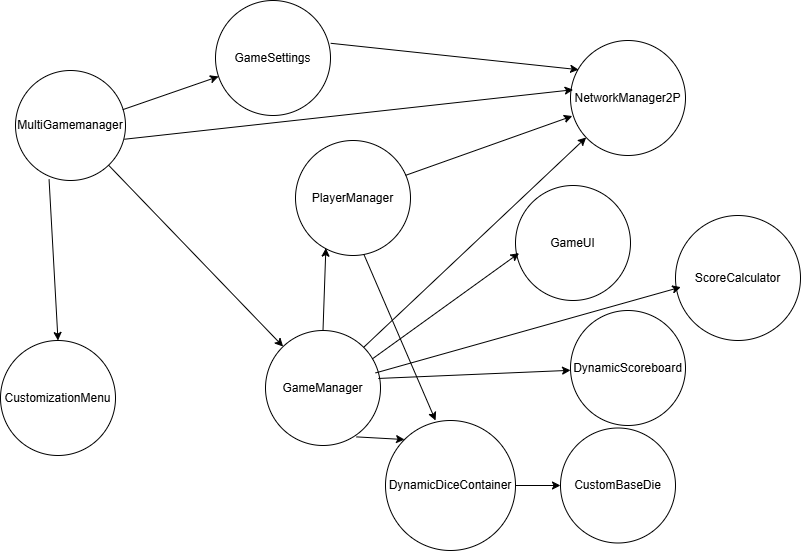
\includegraphics[width=0.7\textwidth]{UsesHierarchy.png}
\caption{Use hierarchy among modules}
\label{FigUH}
\end{figure}

%\section*{References}

\section{User Interfaces}

\wss{Design of user interface for software and hardware.  Attach an appendix if
needed. Drawings, Sketches, Figma}

\section{Design of Communication Protocols}

\wss{If appropriate}

\section{Timeline}

\wss{Schedule of tasks and who is responsible}

\wss{You can point to GitHub if this information is included there}

\bibliographystyle {plainnat}
\bibliography{../../../refs/References}

\newpage{}

\end{document}